\documentclass[
	10pt,								% globale Schriftgröße
	parskip=half-,						% setzt Absatzabstand hoch
	paper=a4,							% Format
	english,ngerman,					% lädt Sprachpakete
	]{scrartcl}							% Dokumentenklasse

% //////////////////// Pakete laden ////////////////////
\usepackage{amsmath}			% MUSS vor fontspec geladen werden
\usepackage{mathtools}			% modifiziert amsmath
\usepackage{amssymb}			% mathematische symbole, für \ceckmarks
\usepackage{amsthm}				% für proof
\usepackage{mathrsfs}			% für \mathscr
\usepackage{latexsym}
\usepackage{marvosym}				% für Lightning

\usepackage{fontspec} 			% funktioniert nur mit den neueren Compilern z.B. XeLaTeX
\usepackage{microtype}			% für bessere Worttrennung
\usepackage[ngerman]{babel} 	% Spracheinstellung
\usepackage{lmodern}			% verändert verwendete Schriftart, damit sie weniger pixelig ist

\usepackage{verbatim}
\usepackage{listings}			% Für Quellcode

\usepackage{graphicx}
\usepackage{tabularx}			% für Tabellen mit gleicher Spaltenbreite und automatischen Umbrüchen
\usepackage{fullpage}
\usepackage{multirow}			% für multirow in tabulars
\usepackage{rotate}
\usepackage[cmyk,table]{xcolor} % um Farben zu benutzen, kann mehr als das Paket color
\usepackage[					% Verlinkungen
	colorlinks,					% farbige Schrift, statt farbiger Rahmen
	linktocpage,				% verlinkt im Abb.Verzeichnis Seitenzahl statt Bildunterschrift
	linkcolor=blue				% setzt Farbe der Links auf blau
	]{hyperref}					% nur für digitale Anwendungen, url = "http://www.example.com"
\usepackage{url}				% für Webadressen wie e-mail usw.: "\url{http://www.example.com}"

\usepackage{enumerate}			% für versch. Aufzählungezeichen wie z.B. a)
\usepackage{xspace}				% folgt ein Leerzeichen nach einem \Befehl, wird es nicht verschluckt.
\usepackage{cancel}				% für das Durchstreichen u.a. in Matheformeln mit \cancel
\usepackage{float}              % zum Forcieren der Position von figure-Umgebungen

% zum Zeichnen (u.a. von Graphen)
\usepackage{fp}
\usepackage{tikz}
\usetikzlibrary{tikzmark}			% für \tikzmark{toRemember}
\usetikzlibrary{positioning}	% verbesserte Positionierung der Knoten
\usetikzlibrary{automata}		% für Automaten (GTI)
\usetikzlibrary{arrows}
\usetikzlibrary{shapes}
\usetikzlibrary{decorations.pathmorphing}
\usetikzlibrary{decorations.pathreplacing}
\usetikzlibrary{decorations.shapes}
\usetikzlibrary{decorations.text}

% //////////////////// Syntaxhighlighting ////////////////////
\lstloadlanguages{Python, Haskell, [LaTeX]TeX, Java}
\lstset{
   basicstyle=\footnotesize\ttfamily,	% \scriptsize the size of the fonts that are used for the code
   backgroundcolor = \color{bgcolour},	% legt Farbe der Box fest
   breakatwhitespace=false,	% sets if automatic breaks should only happen at whitespace
   breaklines=true,			% sets automatic line breaking
   captionpos=t,				% sets the caption-position to bottom, t for top
   commentstyle=\color{codeblue}\ttfamily,% comment style
   frame=single,				% adds a frame around the code
   keepspaces=true,			% keeps spaces in text, useful for keeping indentation
							% of code (possibly needs columns=flexible)
   keywordstyle=\bfseries\ttfamily\color{codepurple},% keyword style
   numbers=left,				% where to put the line-numbers;
   							% possible values are (none, left, right)
   numberstyle=\tiny\color{codegreen},	% the style that is used for the line-numbers
   numbersep=5pt,			% how far the line-numbers are from the code
   stepnumber=1,				% nummeriert nur jede i-te Zeile
   showspaces=false,			% show spaces everywhere adding particular underscores;
							% it overrides 'showstringspaces'
   showstringspaces=false,	% underline spaces within strings only
   showtabs=false,			% show tabs within strings adding particular underscores
   flexiblecolumns=false,
   tabsize=1,				% the step between two line-numbers. If 1: each line will be numbered
   stringstyle=\color{orange}\ttfamily,	% string literal style
   numberblanklines=false,				% leere Zeilen werden nicht mitnummeriert
   xleftmargin=1.2em,					% Abstand zum linken Layoutrand
   xrightmargin=0.4em,					% Abstand zum rechten Layoutrand
   aboveskip=2ex, 
}

\lstdefinestyle{py}{
   language=Python,
}
\lstdefinestyle{hs}{
   language=Haskell,
}
\lstdefinestyle{tex}{
	language=[LaTeX]TeX,
	escapeinside={\%*}{*)},     % if you want to add LaTeX within your code
	texcsstyle=*\bfseries\color{blue},% hervorhebung der tex-Schlüsselwörter
	morekeywords={*,$,\{,\},\[,\],lstinputlisting,includegraphics,
	rowcolor,columncolor,listoffigures,lstlistoflistings,
	subsection,subsubsection,textcolor,tableofcontents,colorbox,
	fcolorbox,definecolor,cellcolor,url,linktocpage,subtitle,
	subject,maketitle,usetikzlibrary,node,path,addbibresource,
	printbibliography},% if you want to add more keywords to the set
     numbers=none,
     numbersep=0pt,
     xleftmargin=0.4em,
}

\lstdefinestyle{java}{
	language=Java,
	extendedchars=true,		% lets you use non-ASCII characters;
   						% for 8-bits encodings only, does not work with UTF-8
}

\lstdefinelanguage[x64]{Assembler}     % add a "x64" dialect of Assembler
   [x86masm]{Assembler} % based on the "x86masm" dialect
   % with these extra keywords:
   {morekeywords={CDQE,CQO,CMPSQ,CMPXCHG16B,JRCXZ,LODSQ,MOVSXD, %
                  POPFQ,PUSHFQ,SCASQ,STOSQ,IRETQ,RDTSCP,SWAPGS, %
                  rax,rdx,rcx,rbx,rsi,rdi,rsp,rbp, %
                  r8,r8d,r8w,r8b,r9,r9d,r9w,r9b}
}					% for 8-bits encodings only, does not work with UTF-8

\lstdefinestyle{c}{
	language=c,
	extendedchars=true,		% for 8-bits encodings only, does not work with UTF-8
}

% //////////////////// eigene Kommandos ////////////////////
\newcommand\FU{Freie Universität Berlin\xspace}% benötigt package xspace
\newcommand\gdw{g.\,d.\,w.\xspace}
\newcommand\oBdA{o.\,B.\,d.\,A.\xspace}
\newcommand{\Eu}{\texteuro}
\newcommand\N{\mathbb{N}\xspace}
\newcommand\Q{\mathbb{Q}\xspace}
\newcommand\R{\mathbb{R}\xspace}
\newcommand\Z{\mathbb{Z}\xspace}
\newcommand\ohneNull{\ensuremath{\backslash\lbrace 0\rbrace}}% \{0}
\let\dhALT\dh	% Schreibt Befehl \dh in \dhALT um
\renewcommand\dh{d.\,h.\xspace}	%renew überschreibt command \dh
\newcommand\Bolt{\;\text{\LARGE\raisebox{-0.3em}{\Lightning}\normalsize}\xspace}% Blitz
\newcommand\zz{\ensuremath{\raisebox{+0.25ex}{Z}% zu zeigen
			\kern-0.4em\raisebox{-0.25ex}{Z}%
			\;\xspace}}
\newcommand{\from}{\ensuremath{\colon}}
\newcommand{\floor}[1]{\lfloor{#1}\rfloor}
\newcommand{\ceil}[1]{\lceil{#1}\rceil}
 \renewcommand{\L}{\ensuremath{\mathcal{L}}\xspace}
 \renewcommand{\P}{\ensuremath{\mathcal{P}}\xspace}
 \newcommand{\NL}{\ensuremath{\mathcal{N}\kern-0.2em\mathcal{L}}\xspace}
 \newcommand{\NP}{\ensuremath{\mathcal{NP}}\xspace}

% //////////////////// Mathefunktionen ////////////////////
\DeclareMathOperator{\Landau}{\mathcal{O}}
\DeclareMathOperator{\True}{True}
\DeclareMathOperator{\False}{False}

% //////////////////// eigene Theoreme ////////////////////
\newtheorem{theorem}{Satz}
\newtheorem{corollary}[theorem]{Folgerung}
\newtheorem{lemma}[theorem]{Lemma}
\newtheorem{observation}[theorem]{Beobachtung}
\newtheorem{definition}[theorem]{Definition}
\newtheorem{Literatur}[theorem]{Literatur}
% konfiguriert proof
\makeatletter
\newenvironment{Proof}[1][\proofname]{\par
  \pushQED{\qed}%
  \normalfont \topsep6\p@\@plus6\p@\relax
  \trivlist
  \item[\hskip\labelsep
%         \itshape
        \bfseries
    #1\@addpunct{.}]\ignorespaces
}{%
  \popQED\endtrivlist\@endpefalse
}
\makeatother

% //////////////////// eigene Farben ////////////////////
\let\definecolor=\xdefinecolor
\definecolor{FUgreen}{RGB}{153,204,0}
\definecolor{FUblue}{RGB}{0,51,102}

\definecolor{middlegray}{rgb}{0.5,0.5,0.5}
\definecolor{lightgray}{rgb}{0.8,0.8,0.8}
\definecolor{orange}{rgb}{0.8,0.3,0.3}
\definecolor{azur}{rgb}{0,0.7,1}
\definecolor{yac}{rgb}{0.6,0.6,0.1}
\definecolor{Pink}{rgb}{1,0,0.6}

\definecolor{bgcolour}{rgb}{0.97,0.97,0.97}
\definecolor{codegreen}{rgb}{0,0.6,0}
\definecolor{codegray}{rgb}{0.35,0.35,0.35}
\definecolor{codepurple}{rgb}{0.58,0,0.82}
\definecolor{codeblue}{rgb}{0.4,0.5,1}

% //////////////////// eigene Settings ////////////////////

\textheight = 230mm		% Höhe des Satzspiegels / Layouts
\footskip = 10ex			% Abstand zw. Fußzeile und Grundlinie letzter Textzeile
\parindent 0pt			% verhindert Einrückung der 1. Zeile eines Absatzes
\setkomafont{sectioning}{\rmfamily\bfseries}% setzt Ü-Schriften in Serifen, {disposition}

\newcommand{\dozent}{Lutz Prechelt}
\newcommand{\tutor}{Samuel Domiks}
\newcommand{\tutoriumNo}{02\\Materialien: Latex, Skript}
\newcommand{\ubungNo}{08}
\newcommand{\veranstaltung}{Softwaretechnik}
\newcommand{\semester}{SoSe21}
\newcommand{\studenten}{Jonny Lam \& Thore Brehmer}

% /////////////////////// BEGIN DOKUMENT /////////////////////////
\begin{document}
% /////////////////////// BEGIN TITLEPAGE /////////////////////////
\begin{titlepage}
	\subject{\dozent}
	\title{\veranstaltung, \semester}
	\subtitle{\Large Übung \ubungNo\\ \large\vspace{1ex} TutorIn: \tutor\\ Tutorium \tutoriumNo}
	\author{\studenten}
	\date{\normalsize \today}
\end{titlepage}

\maketitle								% Erstellt das Titelblatt
\vspace*{-10cm}							% rückt Logo an den oberen Seitenrand
\makebox[\dimexpr\textwidth+1cm][r]{	%rechtsbündig und geht rechts 1cm über Layout hinaus
	
\includegraphics[width=0.4\textwidth]{src/fu_logo} % fügt FU-Logo ein
}
% /////////////////////// END TITLEPAGE /////////////////////////

\vspace{7cm}							% Abstand
\rule{\linewidth}{0.8pt}				% horizontale Linie

% /////////////////////// Task 1 /////////////////////////
\section{Begriffe}
\begin{enumerate}[(a)]
    % /////////////////////// a /////////////////////////
    \item {\itshape Erläutern Sie jeweils knapp den wichtigsten Unterschied oder Zusammenhang zwischen ...}
    \begin{enumerate}[1.]
        \item \textbf{Schnittstelle und Signatur}
        \begin{itemize}
            \item Eine \textbf{Schnittstelle} gibt an, welche Methoden in den unterschiedlichen Klassen vorhanden sind oder vorhanden sein müssen. [1]
            \item Eine \textbf{Signatur} definiert die formale Schnittstelle einer Funktion oder Prozedur. Sie besteht aus dem Namen der Funktion sowie Parametern und Rückgabewert. [2]
        \end{itemize}
        
%        \begin{itemize}
%            \item \textbf{Laut Vorlesung:}
%            \begin{itemize}
%                \item Mithilfe einer Schnittstelle sollte man das Modul verstehen können.
%                \item Nur mithilfe einer Schnittstelle kann man von außen auf ein Modul zugreifen. 
%                \item Dabei verbirgt die Schnittstelle die Entwurfsentscheidungen vor der Außenwelt. Gerade  diejenigen Entwurfsentscheidungen, die sich öfter mal ändern. Was bewirkt, dass man bei späteren Änderungen dann meist nur ein Modul verändern muss, weil dessen Schnittstelle trotz der Änderung gleich bleiben kann.
%                \item Die Schnittstelle ist also die Gesamtheit aller relevanten extern sichtbaren Eigenschaften des Moduls. 
%            \end{itemize}
            
%        \end{itemize}
        \item \textbf{Klasse und Komponente}
        \begin{itemize}
            \item Die \textbf{Klasse} dient als Bauplan und beschreibt Attribute (Eigenschaften) und Methoden (Verhaltensweisen) der Objekte.[3] Eine Klasse kann ein Modul sein.
            \item \textbf{Komponente} in 3.
        \end{itemize}
        
        \item \textbf{Komponente und Modul}
        \begin{itemize}
            \item Ein \textbf{Modul} (neuerdings auch \textbf{Komponente} genannt) ist ein hierarchisches Teil vom System. Ein Modul ist also eine Einheit zusammengehörender Programmelemente (z.B. Daten, Datentypen, Klassen, Funktionen etc). Auf den oberen Ebenen nennt man es auch Subsystem. (Module sollten möglichst geringe Kopplung mit anderen Modulen haben.)
        \end{itemize}
        
        \item \textbf{Kohäsion und Kopplung}
        \begin{itemize}
            \item \textbf{Kohäsion und Kopplung} sind ein Maß um die Komplexität ihrer Software zu analysieren. Es beschreibt die Komplexität der Beziehungen zwischen den Klassen und die innere Zusammengehörigkeit innerhalb der Klassen.[6]
            \item \textbf{Kohäsion} beschreibt wie gut eine Programmeinheit eine logische Aufgabe oder Einheit abbildet. In einem System mit starker Kohäsion ist jede Programmeinheit (eine Methode, eine Klasse oder ein Modul) verantwortlich für genau eine wohldefinierte Aufgabe oder Einheit. [4]
            \item Unter \textbf{Kopplung} versteht man die Verknüpfung von verschiedenen Systemen, Anwendungen oder Softwaremodulen sowie ein Maß, das die Stärke dieser Verknüpfung bzw. der daraus resultierenden Abhängigkeit beschreibt.[5]
        \end{itemize}
    \end{enumerate}
  
    % /////////////////////// b /////////////////////////
    \item {\itshape Erklären Sie die offensichtlichsten Unterschiede zwischen Komponenten, Entwurfsmustern und Architekturstilen.}
    \begin{itemize}
        \item Ein \textbf{Architekturstil} beschreibt welche Teile das System hat, wie diese zusammenspielen und wie dadurch die Funktionalen und nicht Funktionalen Anforderungen erfüllt werden.
        \item \textbf{Komponenten} sind Teile des Systems, welche durch zerlegen des Systems entstehen.
        \item \textbf{Entwurfsmuster} sind bewährte Lösungsschablonen für wiederkehrende Entwurfsprobleme/Teilprobleme eines Systems in der Softwarearchitektur.[12]
    \end{itemize}


    % /////////////////////// c /////////////////////////
    \item {\itshape Recherchieren Sie das Entwurfsmuster Einzelstück (engl.singleton). Denken Sie wie immer daran Ihre Quellen anzugeben.}
   \begin{enumerate}[1.]
        \item {\itshape Erläutern Sie das Entwurfsmuster, d.h. welches Problem löst es wie?}
        \begin{itemize}
            \item Das \textbf{Singleton} findet Verwendung, wenn nur ein Objekt zu einer Klasse existieren darf und ein einfacher Zugriff auf dieses Objekt benötigt wird (oder das einzige Objekt durch Unterklassenbildung spezialisiert werden soll.)[7]
        \end{itemize}
        
        \item {\itshape Illustrieren Sie das Entwurfsmuster indem Sie drei hypothetische Beispiele für seine Verwendung formulieren.}
        \begin{itemize}
            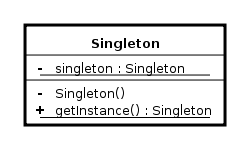
\includegraphics[width=0.35\textwidth]{src/u8/250px-Singleton_UML_class_diagram.svg.png}[7]
            \item \textbf{Verwendungs Beispiele:} 
            \begin{enumerate}[1.]
                \item Für die Darstellung einer Zentralbank.
                \item Für die Darstellung eines Königs.
                \item Für die Darstellung eines Gottes (für monotheistische Religionen).
                \\(Da es für jedes dieser Beispiele höchstens ein Objekt geben kann)
            \end{enumerate}
         \end{itemize}

        
        \item {\itshape Zu welcher Klasse der in der Vorlesung vorgestellten Entwurfsmustertaxonomie (pattern taxonomy) gehört dieses Muster und warum?}
        \begin{itemize} 
            \item  Da beim \textbf{Singleton} von einer Klasse nur ein einziges Objekt erzeugt werden darf, passt es gut zum \textbf{Erzeugungsmuster}, da das Ziel des Erzeugungsmuster ist das System unabhängig davon zu machen wie seine Objekte erzeugt, komponiert und repräsentiert werden.
        \end{itemize}

    \end{enumerate}
    
    % /////////////////////// d /////////////////////////
    \item {\itshape Charakterisieren und vergleichen Sie die folgenden Entwurfsmuster: Stellvertreter(Proxy), Adapter (Adapter), Fassade (Facade), Brücke (Bridge).}
    \begin{itemize}
        \item \textbf{Stellvertreter(Proxy):} Umschließt ein anderes Objekt und kontrolliert den Zugriff darauf.[14]
        \item \textbf{Adapter (Adapter):} Umschließt ein Objekt(Schnittstelle) und stelle eine andere Schnittstelle dafür zur Verfügung. Entweder weil der Client sonst nicht darauf zugreifen kann, oder um die Schnittstelle zu vereinfachen. Dadurch muss weder beim Client und noch beim Adaptee was verändert werden, nur beim Adapter.[13]
        \item \textbf{Fassade (Facade):} Vereinfacht eine Schnittstelle.[15]
        \item \textbf{Brücke (Bridge)} Erlaubt separate Entwicklung von Abstraktions- und Implementierungshierarchien.[16]

    \end{itemize}
    
\end{enumerate}



% /////////////////////// Task 2 /////////////////////////
\section{Entwurfsmuster für eigene Software-Idee}
\begin{enumerate}[(a)]
    % /////////////////////// a /////////////////////////
    \item {\itshape Überlegen Sie sich, welches der in der Vorlesung vorgestellten Entwurfsmuster Sie in Ihrer zu entwickelnden Software sinnvoll einsetzen können (außer dem Singleton und dem Adapter). Stellen Sie die Charakteristika des gewählten Entwurfsmusters heraus (d.h. welches Problem löst es wie) und begründen Sie, warum und wofür das Muster in Ihrem Kontext geeignet ist.}
    \begin{itemize}
        \item Das \textbf{Strategy} Entwurfsmuster wird verwendet, um eine austauschbare Familie von Algorithmen zu erstellen, aus der der erforderliche Prozess zur Laufzeit ausgewählt wird. Dadurch kann sich das Verhalten eines Programms je nach Konfigurationsdetails oder Benutzerpräferenzen dynamisch ändern. Es erhöht auch die \underline{Flexibilität}, indem es ermöglicht, dass neue Algorithmen in Zukunft \underline{einfach integriert} werden können.[11]
        \item \textbf{Es löst also folgende Probleme}: ''Wenn man verschiedene Wege hat, etwas zu machen, dann soll man diese \underline{frei hinzufügen}, \underline{benutzen} oder \underline{austauschen} können, je nachdem, was gerade gebraucht wird.''[10]
        
        \item \textbf{Für unseren Kontext ist es geeignet}, da wir mit unseren Digitalen Bon App Bons mithilfe von \underline{verschiedenen Verfahren} einscannen wollen. Die verschiedenen Scans benötigen unterschiedliche Scan- sowie Decode Methoden (Scan zum einlesen der Daten und Decode um die Daten auch verwenden zu können). Das Ergebnis von verschiedenen Scan Methoden könnten aber von einer einzigen Decode Methode benutzt werden. (Bsp. Das Ergebnis von Scan Dropbox und Scan GoogleDrive kann von DecodeHtml benutzt werden)

        \item Um \underline{gute Skalierbarkeit} (vielleicht werden zukünftig neue Scan Methoden verwendet) und \underline{gute Code leserlichkeit} zu ermöglichen (anstatt für jeden Scan+Decode eine einzelne neue Klasse) haben wir uns für das Strategy Entwurfsmuster entschieden. 

    \end{itemize}
    
    % /////////////////////// b /////////////////////////
    \item {\itshape Stellen Sie das Entwurfsmuster in seiner allgemeinen Form, d.h. unter Verwendung der Rollennamen, in UML-Notation dar. Recherchieren Sie nach Bedarf und geben Sie in jedem Fall Ihre Quellen an.}
    \begin{center}
       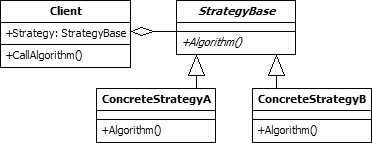
\includegraphics[width=0.5\textwidth]{src/u8/Strategy.png}[11] 
    \end{center}
    


    % /////////////////////// c /////////////////////////
    \item {\itshape Übertragen Sie nun das gewählte Entwurfsmuster in Ihren  Kontext und stellen das Ergebnis ebenfalls als UML-Diagramm dar.}
    \begin{center}
       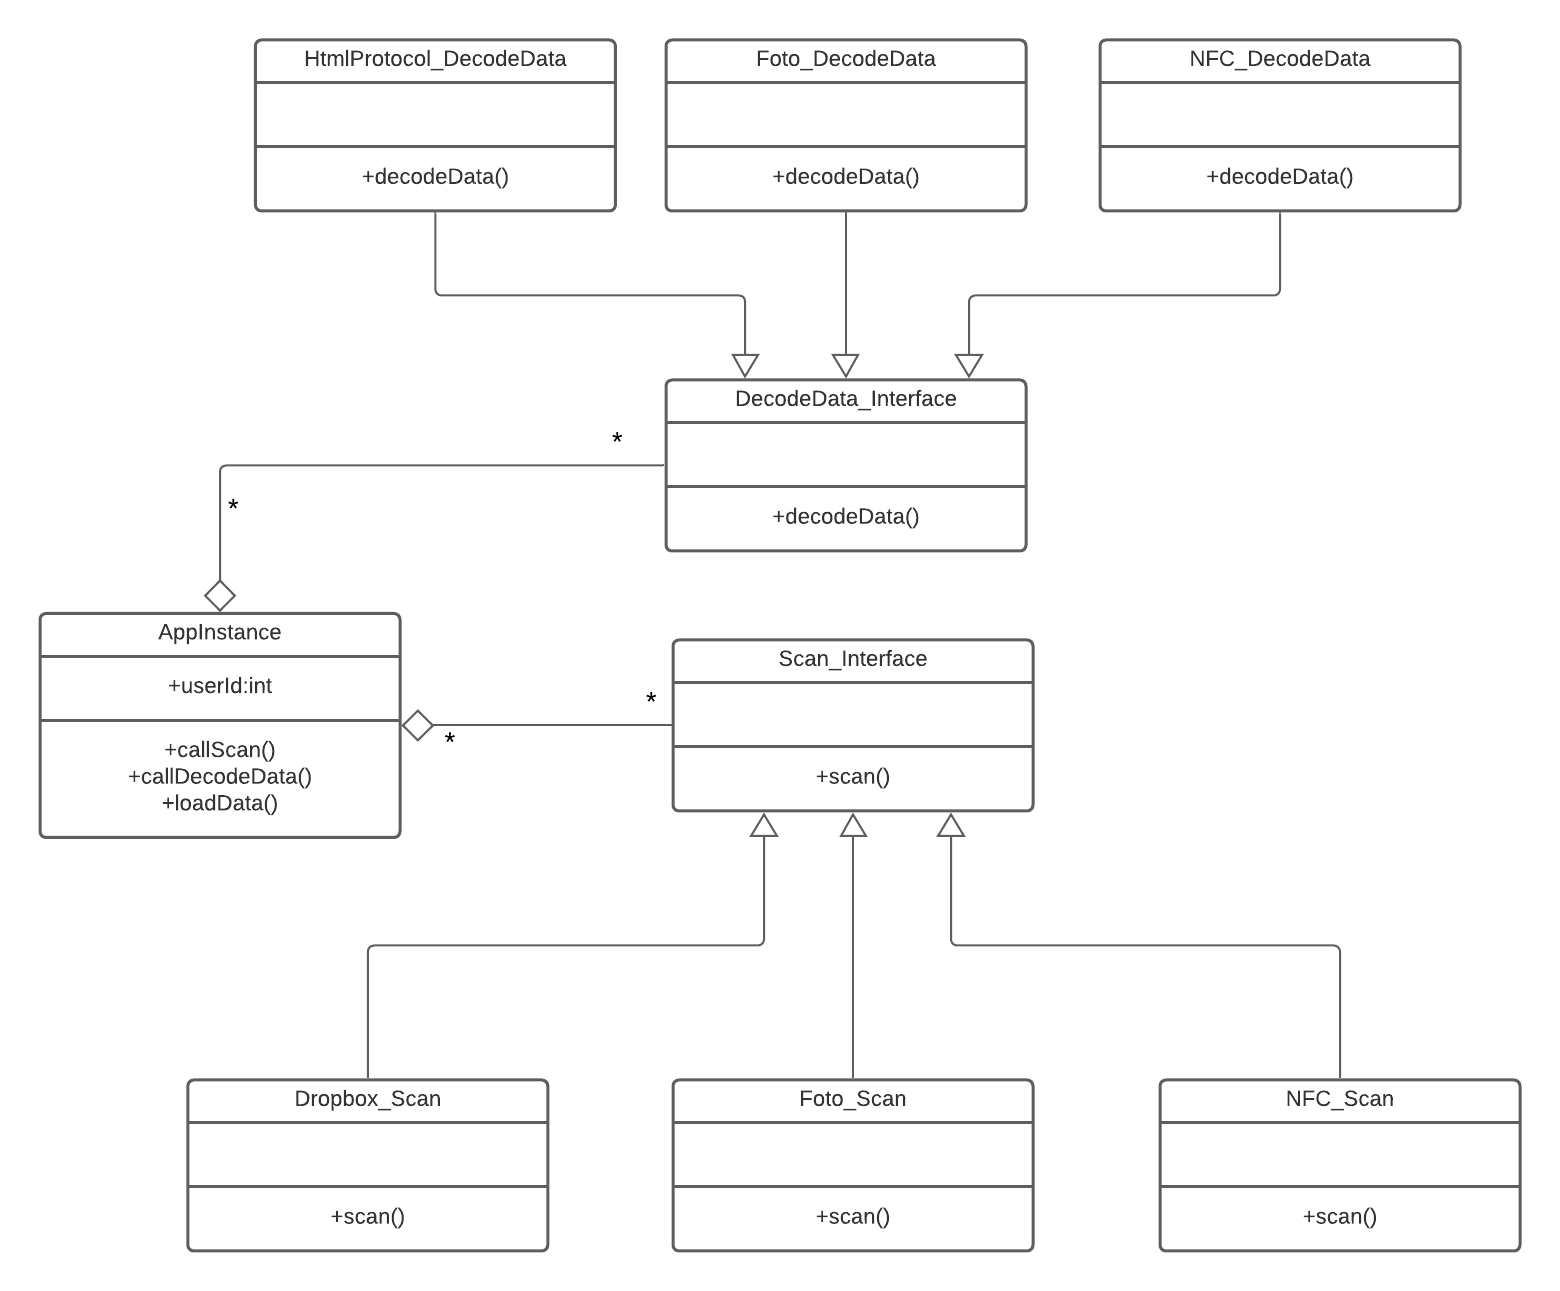
\includegraphics[width=1\textwidth]{src/u8/task2/8_2.png} 
    \end{center}

    % /////////////////////// d /////////////////////////
    \item {\itshape Nicht alle Aspekte eines Entwurfsmusters lassen sich bequem in einem UML-Diagrammausdrücken. Implementieren Sie (in Java oder Pseudocode) in Ansätzen die Verwendung des Entwurfsmusters in Ihrem Kontext. Erstellen Sie die für das Muster notwendigen Schnittstellen und Klassen, mit den jeweils relevanten Code stellen, d.h. zumindest angedeutete Daten- und Kontrollstrukturen (leere Methodenrümpfe reichen in aller Regel nicht aus). Schreiben Sie ausdrücklich keinen Code, der über das bloße Entwurfs-muster hinaus geht!}
    \\
    \begin{itemize}
    \newpage
    \lstinputlisting[language=java]{src/u8/task2/AppInstance.java}
    \lstinputlisting[language=java]{src/u8/task2/Scan_Interface.java}
    \lstinputlisting[language=java]{src/u8/task2/NFC_Scan.java}
    \lstinputlisting[language=java]{src/u8/task2/Foto_Scan.java}
    \lstinputlisting[language=java]{src/u8/task2/Dropbox_Scan.java}
    \newpage \lstinputlisting[language=java]{src/u8/task2/DecodeData_Interface.java}
    \lstinputlisting[language=java]{src/u8/task2/NFC_DecodeData.java}
    \lstinputlisting[language=java]{src/u8/task2/Foto_DecodeData.java}
    \lstinputlisting[language=java]{src/u8/task2/HtmlProtocol_DecodeData.java}

    \end{itemize}

\end{enumerate}
\newpage
% /////////////////////// Task 3 /////////////////////////
\section{: Adapter-Entwurfsmuster anwenden}
\begin{enumerate}[(a)]
    % /////////////////////// a /////////////////////////
    \item {\itshape \textbf{Aufgabe:} Implementieren Sie eine neue Klasse (etwa „Storage“) mit einer einzigen Methode (etwa „store“), die Dateinamen und Inhalt erhält und Ihre alte Filesystem-Klasse wiederverwendet – ohne diese zu verändern!}
    \begin{itemize}
        \lstinputlisting[language=java]{src/u8/Storage_1.java}
        \lstinputlisting[language=java]{src/u8/NotepadMinusMinus_1.java}
    \end{itemize}
  
    % /////////////////////// b /////////////////////////
    \item {\itshape Das klassische Adapter-Muster kennt die folgenden vier Rollen: Client, Target, Adapter und Adaptee. Geben Sie für jede dieser Rollen an, durch welche der Klassen Ihrer Implementierung diese ausgefüllt wird?}
    \begin{itemize}
        \item Client \rightarrow NotepadMinusMinus
        \item Target \rightarrow None
        \item Adapter \rightarrow Storage
        \item Adaptee \rightarrow Filesystem
    \end{itemize}
   

    % /////////////////////// c /////////////////////////
    \item {\itshape Nutzen Sie das Dropbox-SDK, um Ihren Editor um eine Speicher-Option zu erweitern. Wie schon bei der Filesystem-Wiederverwendung sollen (bzw. können) Sie den Dropbox-Quellcode nicht verändern. Schreiben Sie also einen weiteren Adapter hierfür. Um in der NotepadMinusMinus-Klasse nicht direkt von einem der beiden Adapter (einen für das lokale Dateisystem, einen für Dropbox) abzuhängen, führen Sie bitte ein Interface ein (etwa „IStorage“), das die beiden Adapter jeweils implementieren. Um in der NotepadMinusMinus-Klasse davon Gebrauch machen zu können, implementieren Sie bitte eine Setter-Methode und verwenden den übergebenen Wert in der bereits existierenden save()-Methode:}
    \newpage
    \begin{itemize}
        \lstinputlisting[language=java]{src/u8/IStorage_2.java}
        \lstinputlisting[language=java]{src/u8/Storage_2.java}
        \lstinputlisting[language=java]{src/u8/StorageDropbox_2.java}
        \lstinputlisting[language=java]{src/u8/NotepadMinusMinus_2.java}
    \end{itemize}
   
   
    % /////////////////////// d /////////////////////////
    \item {\itshape Analog zu Aufgabe b): Wie sieht die Rollenverteilung (also Client, Target, Adapter, Adaptee) auf die Klassen und Schnittstellen der zweiten Implementierung aus? Bedenken Sie, dass Sie nun zwei Exemplare des Adapter-Musters vorliegen haben.}
    \begin{itemize}
        \item Client \rightarrow NotepadMinusMinus
        \item Target \rightarrow IStorage
        \item Adapter \rightarrow Storage, StorageDropbox
        \item Adaptee \rightarrow Filesystem, DbxClient
    \end{itemize}
    
    % /////////////////////// e /////////////////////////
    \item {\itshape In der zweiten Implementierung „weiß“ die zentrale Editor-Klasse zur Kompilierzeit nicht, welche Implementierung des Storage-Interfaces sie konkret benutzen wird. Diese wird erst zur Laufzeit über die setStorage()-Methode „hineingereicht“.Recherchieren Sie die Idee der „Dependency Injection“ (Quellen angeben). Welche Vorteile halt dieses Entwurfsprinzip? Welche Nachteile?}
    \begin{itemize}
        \item Als \textbf{Dependency Injection} wird in der objektorientierten Programmierung ein Entwurfsmuster bezeichnet, welches die Abhängigkeiten eines Objekts zur Laufzeit reglementiert: Benötigt ein Objekt beispielsweise bei seiner Initialisierung ein anderes Objekt, ist diese Abhängigkeit an einem zentralen Ort hinterlegt – es wird also nicht vom initialisierten Objekt selbst erzeugt.[8]

        \textbf{Vorteile [9]:}
        \item \textbf{Flexibilität:} Nur das Verhalten des Clients ist festgelegt, der Client kann auf alles reagieren was die vom Client erwartete interne Schnittstelle unterstützt.
        \item \textbf{Systeme können ohne Neukompilierung neu konfiguriert werden}, da die Konfigurationsdaten ein Konfigurationsdateien ausgelagert werden können. 
        \item \textbf{Wiederverwendbarkeit,Testbarkeit und Wartbarkeit}, da man eine ganze Implementierung entfernen kann um Auswirkungen von Designänderung und fehlern zu isolieren.
        \item \textbf{Gleichzeitige oder unabhängige Entwicklung}, da Entwickler nur die Schnittstelle kennen müssen um unabhängig voneinander Klassen zu entwickeln.\\
        \textbf{Nachteile[9]:}
        \item \textbf{Lesen von Code wird erschwert}, da das Verhalten von der Konstruktion getrennt wird. Entwickler müssen auf weitere Dateien verweisen um die Leistung eine Systems zu verfolgen.
        \item \textbf{Mehr Entwicklungsaufwand im Voraus erforderlich.} Man weiß im Vorhinein nicht wann und wo es benötigt wird, sondern man muss anfragen dass es injiziert wird und dann sicherstellen, dass es wirklich injiziert wurde.
        \item \textbf{Schwierig in die Verknüpfung zwischen Klassen zu gelangen.}
    \end{itemize}
    
\end{enumerate}



% /////////////////////// Quellen /////////////////////////
\section{Quellen}
\begin{enumerate}[{[1]}]
    \item ``Schnittstelle (Objektorientierung)'', \url{https://de.wikipedia.org/wiki/Schnittstelle_(Objektorientierung)} .
[aufgerufen am 01.06.2021]
    \item ``Signatur (Programmierung)'', \url{https://de.wikipedia.org/wiki/Signatur_(Programmierung)} [aufgerufen am 01.06.2021]
    \item ``Klasse (Objektorientierung)'', \url{https://de.wikipedia.org/wiki/Klasse_(Objektorientierung)} [aufgerufen am 01.06.2021]
    \item ``Kohäsion (Informatik)'', \url{https://de.wikipedia.org/wiki/Kohäsion_(Informatik)} [aufgerufen am 01.06.2021]
    \item ``Kopplung (Softwareentwicklung)'', \url{https://de.wikipedia.org/wiki/Kopplung_(Softwareentwicklung)} [aufgerufen am 01.06.2021]
    \item ``Kohäsion und Kopplung'', \url{https://sites.google.com/site/koesterprogramming/home/softwareentwicklung/kohaesion-und-kopplung} [aufgerufen am 01.06.2021]
    \item ``Singleton (Entwurfsmuster)'', \url{https://de.wikipedia.org/wiki/Singleton_(Entwurfsmuster)} [aufgerufen am 01.06.2021]
    \item ``Dependency Injection''
    \url{https://de.wikipedia.org/wiki/Dependency_Injection} [aufgerufen am 04.06.2021]    
    \item ``Dependency Injection Vorteile\_und\_Nachteile''
    \url{https://de.wikipedia.org/wiki/Dependency_Injection#Vorteile_und_Nachteile} [aufgerufen am 04.06.2021]
    \item ``Vorlesung 12'', (page 26/42) 
    \item ``Strategy Design Pattern'', 
    \url{http://www.blackwasp.co.uk/Strategy.aspx} [aufgerufen am 05.06.2021]
    \item ``Entwurfsmuster'', 
    \url{https://de.wikipedia.org/wiki/Entwurfsmuster} [aufgerufen am 05.06.2021]
    \item ``Adapter Design Pattern'', 
    \url{http://www.blackwasp.co.uk/Adapter.aspx} [aufgerufen am 05.06.2021]
    \item ``Proxy Design Pattern'', 
    \url{http://www.blackwasp.co.uk/Proxy.aspx} [aufgerufen am 05.06.2021]
    \item ``Facade Design Pattern'', 
    \url{http://www.blackwasp.co.uk/Facade.aspx} [aufgerufen am 05.06.2021]
    \item ``Bridge Design Pattern'', 
    \url{http://www.blackwasp.co.uk/Bridge.aspx} [aufgerufen am 05.06.2021]
    

\end{enumerate}

\end{document}